Containers are types that represent collections of elements. These collections can be implemented based on a variety of data structures, each with different semantics: lists, queues, trees, and so on. The standard library provides three categories of containers:

\begin{itemize}
\item
Sequence containers: vector, deque, list, array, and forward\_list

\item
Associative containers: set, map, multiset, and multimap

\item
Unordered associative containers: unordered\_set, unordered\_map, unordered\_multiset, and unordered\_multimap
\end{itemize}

In addition to this, there are also container adaptors that provide a different interface for sequence containers. This category includes the stack, queue, and priority\_queue classes. Finally, there is a class called span that represents a non-owning view over a contiguous sequence of objects.

The rationale for these containers to be templates was presented in Chapter 1, Introduction to Templates. You don’t want to write the same implementation again and again for each different type of element that you need to store in a container. Arguably, the most used containers from the standard library are the following:

\begin{itemize}
\item
vector: This is a variable-size collection of elements stored contiguously in memory. It’s the default container you would choose, provided no special requirements are defined. The internal storage expands or shrinks automatically as needed to accommodate the stored elements. The vector allocates more memory than needed so that the risk of having to expand is low. The expansion is a costly operation because new memory needs to be allocated, the content of the current storage needs to be copied to the new one, and lastly, the previous storage needs to be discarded. Because elements are stored contiguously in memory, they can be randomly accessed by an index in constant time.

\item
array: This is a fixed-size collection of elements stored contiguously in memory. The size must be a compile-time constant expression. The semantics of the array class is the same as a structure holding a C-style array (T[n]). Just like the vector type, the elements of the array class can be accessed randomly in constant time.

\item
map: This is a collection that associates a value to a unique key. Keys are sorted with a comparison function and the map class is typically implemented as a red-black tree. The operations to search, insert, or remove elements have logarithmic complexity.

\item
set: This is a collection of unique keys. The keys are the actual values stored in the container; there are no key-value pairs as in the case of the map class. However, just like in the case of the map class, set is typically implemented as a red-black tree that has logarithmic complexity for searching, inserting, and the removing of elements.
\end{itemize}

Regardless of their type, the standard containers have a few things in common:

\begin{itemize}
\item
Several common member types

\item
An allocator for storage management (with the exception of the std::array class)

\item
Several common member functions (some of them are missing from one or another container)

\item
Access to the stored data with the help of iterators
\end{itemize}

The following member types are defined by all standard containers:

\begin{lstlisting}[style=styleCXX]
using value_type = /* ... */;
using size_type = std::size_t;
using difference_type = std::ptrdiff_t;
using reference = value_type&;
using const_reference = value_type const&;
using pointer = /* ... */;
using const_pointer = /* ... */;
using iterator = /* ... */;
using const_iterator = /* ... */;
\end{lstlisting}

The actual types these names are aliasing may differ from container to container.

For instance, for std::vector, value\_type is the template argument T, but for std::map, value\_type is the std::pair<const Key, T> type. The purpose of these member types is to help with generic programming. Except for the std::array class, which represents an array of a size known at compile time, all the other containers allocate memory dynamically. This is controlled with the help of an object called an allocator. Its type is specified as a type template parameter, but all containers default it to std::allocator if none is specified. This standard allocator uses the global new and delete operators for allocating and releasing memory. All constructors of standard containers (including copy and move constructors) have overloads that allow us to specify an allocator.

There are also common member functions defined in the standard containers. Here are some examples:

\begin{itemize}
\item
size, which returns the number of elements (not present in std::forward\_list).

\item
empty, which checks whether the container is empty.

\item
clear, which clears the content of the container (not present in std::array, std::stack, std::queue, and std::priority\_queue).

\item
swap, which swaps the content of the container objects.

\item
begin and end methods, which return iterators to the beginning and end of the container (not present in std::stack, std::queue, and std::priority\_queue, although these are not containers but container adaptors).
\end{itemize}

The last bullet mentions iterators. These are types that abstract the details of accessing elements in a container, providing a uniform way to identify and traverse the elements of containers. This is important because a key part of the standard library is represented by general-purpose algorithms. There are over one hundred such algorithms, ranging from sequence operations (such as count, count\_if, find, and for\_each) to modifying operations (such as copy, fill, transform, rotate, and reverse) to partitioning and sorting (partition, sort, nth\_element, and more) and others. Iterators are key for ensuring they work generically. If each container had different ways to access its elements, writing generic algorithms would be virtually impossible.

Let’s consider the simple operation of copying elements from one container to another. For instance, we have a std::vector object and we want to copy its elements to a std::list object. This could look as follows:

\begin{lstlisting}[style=styleCXX]
std::vector<int> v {1, 2, 3};
std::list<int> l;

for (std::size_t i = 0; i < v.size(); ++i)
	l.push_back(v[i]);
\end{lstlisting}

What if we want to copy from a std::list to a std::set, or from a std::set to a std::array? Each case would require different kinds of code. However, generalpurpose algorithms enable us to do this in a uniform way. The following snippet shows such an example:

\begin{lstlisting}[style=styleCXX]
std::vector<int> v{ 1, 2, 3 };

// copy vector to vector
std::vector<int> vc(v.size());
std::copy(v.begin(), v.end(), vc.begin());

// copy vector to list
std::list<int> l;
std::copy(v.begin(), v.end(), std::back_inserter(l));

// copy list to set
std::set<int> s;
std::copy(l.begin(), l.end(), std::inserter(s, s.begin()));
\end{lstlisting}

Here we have a std::vector object and we copy its content to another std::vector, but also to a std::list object. Consequently, the content of the std::list object is then copied to a std::set object. For all cases, the std::copy algorithm is used. This algorithm has several arguments: two iterators that define the beginning and end of the source, and an iterator that defines the beginning of the destination. The algorithm copies one element at a time from the input range to the element pointer by the output iterator and then increments the output iterator. Conceptually, it can be implemented as follows:

\begin{lstlisting}[style=styleCXX]
template<typename InputIt, class OutputIt>
OutputIt copy(InputIt first, InputIt last,
			  OutputIt d_first)
{
	for (; first != last; (void)++first, (void)++d_first)
	{
		*d_first = *first;
	}
	return d_first;
}
\end{lstlisting}

\begin{tcolorbox}[breakable,enhanced jigsaw,colback=blue!5!white,colframe=blue!75!black,title={Important Note}]
This algorithm was discussed in Chapter 5, Type Traits and Conditional Compilation, when we looked at how its implementation can be optimized with the help of type traits.
\end{tcolorbox}

Considering the previous example, there are cases when the destination container does not have its content already allocated for the copying to take place. This is the case with copying to the list and to the set. In this case, iterator-like types, std::back\_insert\_iterator and std:insert\_iterator, are used—indirectly through the std::back\_inserter and std::inserter helper functions, for inserting elements into a container. The std::back\_insert\_iterator class uses the push\_back function and std::insert\_iterator uses the insert function.

There are six iterator categories in C++:

\begin{itemize}
\item
Input iterator

\item
Output iterator

\item
Forward iterator

\item
Bidirectional iterator

\item
Random access iterator

\item
Contiguous iterator
\end{itemize}

The contiguous iterator category was added in C++17. All operators can be incremented with the prefix or postfix increment operator. The following table shows the additional operations that each category defines:

% Please add the following required packages to your document preamble:
% \usepackage{multirow}
\begin{table}[H]
\centering
	\begin{tabular}{|l|l|l|}
		\hline
		\textbf{Category}       & \textbf{Properties}               & \textbf{Expressions}                                           \\ \hline
		\multirow{3}{*}{Input}  & Increment single-pass             & \begin{tabular}[c]{@{}l@{}}i++\\ ++i\end{tabular}              \\ \cline{2-3} 
		& Equality/inequality cmparison     & \begin{tabular}[c]{@{}l@{}}i == j\\ i != j\end{tabular}        \\ \cline{2-3} 
		& Can be dereferenced(as an rvalue) & \begin{tabular}[c]{@{}l@{}}*i\\ i-\textgreater{}m\end{tabular} \\ \hline
		Forward                 & Increment multi-pass              & i = j, *j++, *i                                                \\ \hline
		Bidirectional           & Decrement                         & \begin{tabular}[c]{@{}l@{}}--i\\ i--\end{tabular}              \\ \hline
		\multirow{4}{*}{Random-access} &
		Arithmetic operators + and - &
		\begin{tabular}[c]{@{}l@{}}i + n\\ n + i\\ i - n\\ n - i\end{tabular} \\ \cline{2-3} 
		&
		Inequality comparsion(with iterators) &
		\begin{tabular}[c]{@{}l@{}}i \textless j\\ i \textgreater j\\ i \textless{}= j\\ i \textgreater{}= j\end{tabular} \\ \cline{2-3} 
		& Compound assignment               & \begin{tabular}[c]{@{}l@{}}i += n\\ i -= n\end{tabular}        \\ \cline{2-3} 
		& Offset dereference operator       & i{[}n{]}                                                       \\ \hline
		Contiguous &
		\begin{tabular}[c]{@{}l@{}}Logically adjacent elements are physically\\ adjacent in memory.\end{tabular} &
		\\ \hline
		\multirow{2}{*}{Output} & Increment signle-pass             & \begin{tabular}[c]{@{}l@{}}i++\\ ++i\end{tabular}              \\ \cline{2-3} 
		& Can be dereferenced(as an lvalue) & \begin{tabular}[c]{@{}l@{}}*i = v\\ *i++ = v\end{tabular}      \\ \hline
	\end{tabular}
\end{table}

\begin{center}
Table 8.1
\end{center}

With the exception of the output category, each category includes everything about it. That means a forward iterator is an input iterator, a bidirectional iterator is a forward iterator, a random-access iterator is a bidirectional iterator, and, lastly, a contiguous iterator is a random-access iterator. However, iterators in any of the first five categories can also be output iterators at the same time. Such an iterator is called a mutable iterator. Otherwise, they are said to be constant iterators.

The C++20 standard has added support for concepts and a concepts library. This library defines standard concepts for each of these iterator categories. The following table shows the correlation between them:

\begin{table}[H]
\centering
	\begin{tabular}{|l|l|}
		\hline
		\textbf{Iterator category} & \textbf{Concept}              \\ \hline
		Input iterator             & std::input\_iterator          \\ \hline
		Forward iterator           & std::output\_iterator         \\ \hline
		Bidirectional iterator     & std::bidirectional\_iterator  \\ \hline
		Random-access iterator     & std::random\_access\_iterator \\ \hline
		Contiguous iterator        & std::contiguous\_iterator     \\ \hline
		Output iterator            & std::output\_iterator         \\ \hline
	\end{tabular}
\end{table}

\begin{center}
Table 8.2
\end{center}

\begin{tcolorbox}[breakable,enhanced jigsaw,colback=blue!5!white,colframe=blue!75!black,title={Important Note}]
Iterator concepts were briefly discussed in Chapter 6, Concepts and Constraints.
\end{tcolorbox}

All containers have the following members:

\begin{itemize}
\item
begin: It returns an iterator to the beginning of the container.

\item
end: It returns an iterator to the end of the container.

\item
cbegin: It returns a constant iterator to the beginning of the container.

\item
cend: It returns a constant iterator to the end of the container.
\end{itemize}

Some containers also have members that return reverse iterators:

\begin{itemize}
\item
rbegin: It returns a reverse iterator to the beginning of the reversed container.

\item
rend: It returns a reverse iterator to the end of the reversed container.

\item
rcbegin: It returns a constant reverse iterator to the beginning of the reversed container.

\item
rcend: It returns a constant reverse iterator to the end of the reversed container.
\end{itemize}

There are two things that must be well understood to be able to work with containers and iterators:

\begin{itemize}
\item
The end of a container is not the last element of the container but the one past the last.

\item
Reversed iterators provide access to the elements in reverse order. A reversed iterator to the first element of a container is actually the last element of the non-reversed container.
\end{itemize}

To better understand these two points, let’s look at the following example:

\begin{lstlisting}[style=styleCXX]
std::vector<int> v{ 1,2,3,4,5 };

// prints 1 2 3 4 5
std::copy(v.begin(), v.end(),
		  std::ostream_iterator<int>(std::cout, " "));

// prints 5 4 3 2 1
std::copy(v.rbegin(), v.rend(),
		  std::ostream_iterator<int>(std::cout, " "));
\end{lstlisting}

The first call to std::copy prints the elements of the container in their given order. On the other hand, the second call to std::copy prints the elements in their reversed order.

The following diagram illustrates the relationship between iterators and container elements:

\begin{center}
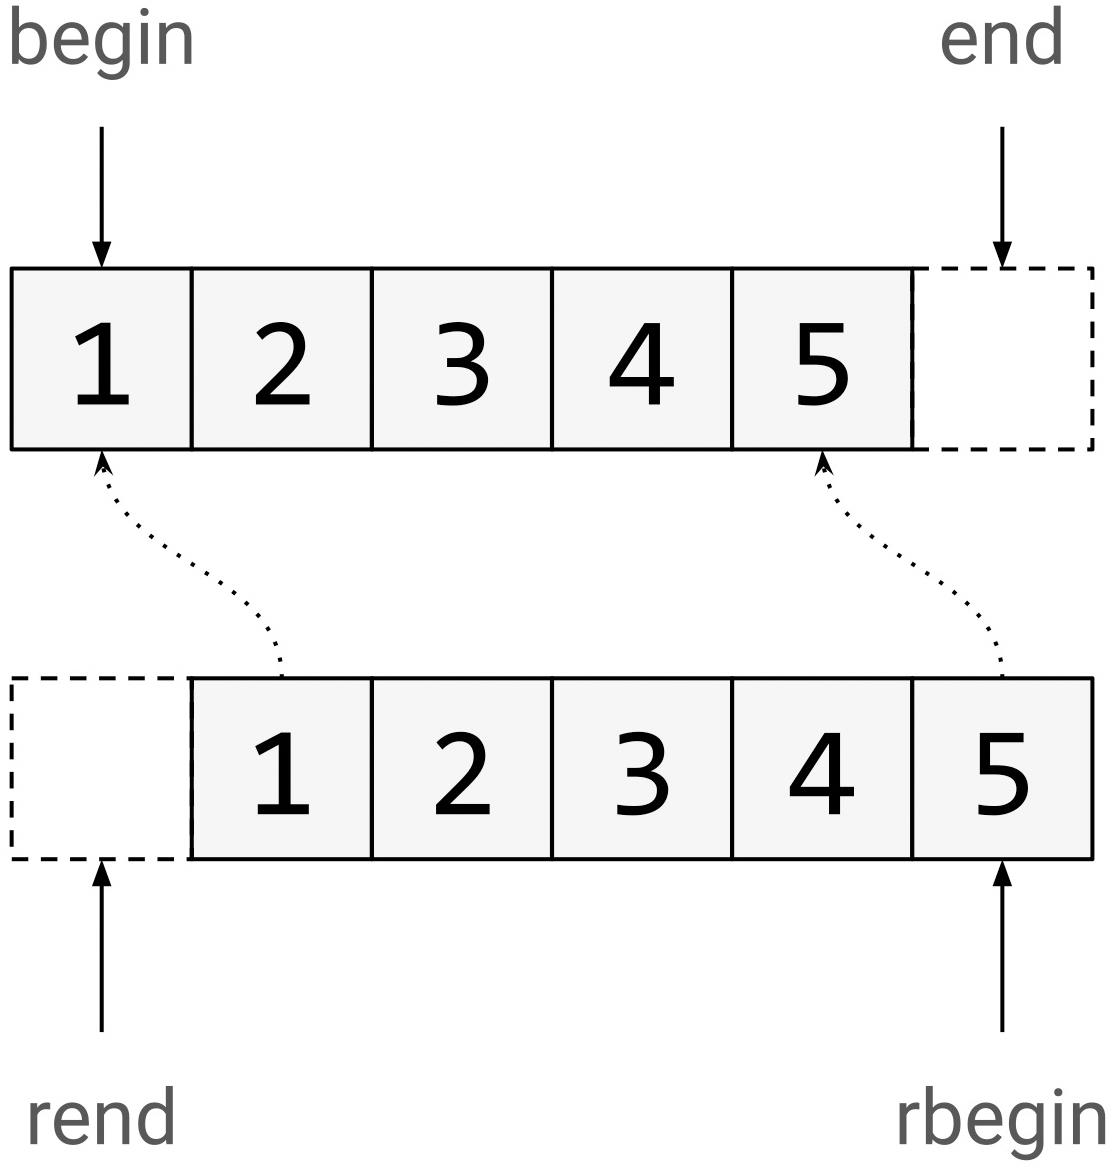
\includegraphics[width=0.3\textwidth]{content/3/chapter8/images/1.png}\\
Figure 8.1
\end{center}

A sequence of elements (regardless of what kind of data structure they are stored in memory) delimited by two iterators (a begin and an end, which is the one past the last element) is called a range. This term is used extensively in the C++ standard (especially with algorithms) and in literature. It is also the term that gave the name to the ranges library in C++20, which will be discussed in Chapter 9, The Ranges Library.

Apart from the set of the begin/end member functions of the standard containers, there are also stand-alone functions with the same name. Their equivalence is presented in the following table:

\begin{table}[H]
\centering
	\begin{tabular}{|l|l|}
		\hline
		\textbf{Member functions}                                    & \textbf{Free functions}                                              \\ \hline
		\begin{tabular}[c]{@{}l@{}}c.begin()\\ c.cbegin()\end{tabular}   & \begin{tabular}[c]{@{}l@{}}std::begin(c)\\ std::cbegin(c)\end{tabular}   \\ \hline
		\begin{tabular}[c]{@{}l@{}}c.end()\\ c.cend()\end{tabular}   & \begin{tabular}[c]{@{}l@{}}std::end(c)\\ std::cend(c)\end{tabular}   \\ \hline
		\begin{tabular}[c]{@{}l@{}}c.rbegin()\\ c.crbegin()\end{tabular} & \begin{tabular}[c]{@{}l@{}}std::rbegin(c)\\ std::crbegin(c)\end{tabular} \\ \hline
		\begin{tabular}[c]{@{}l@{}}c.rend()\\ c.crend()\end{tabular} & \begin{tabular}[c]{@{}l@{}}std::rend(c)\\ std::crend(c)\end{tabular} \\ \hline
	\end{tabular}
\end{table}

\begin{center}
Table 8.3
\end{center}

Although these free functions do not bring much benefit when working with standard containers, they help us in writing generic code that can handle both standard containers and C-like arrays, since all these free functions are overloaded for static arrays. Here is an example:

\begin{lstlisting}[style=styleCXX]
std::vector<int> v{ 1,2,3,4,5 };
std::copy(std::begin(v), std::end(v),
		  std::ostream_iterator<int>(std::cout, " "));

int a[] = { 1,2,3,4,5 };
std::copy(std::begin(a), std::end(a),
		  std::ostream_iterator<int>(std::cout, " "));
\end{lstlisting}

Without these functions, we would have to write std::copy(a, a + 5, …). Perhaps a big benefit of these functions is that they enable us to use arrays with range-based for loops, as follows:

\begin{lstlisting}[style=styleCXX]
std::vector<int> v{ 1,2,3,4,5 };
for (auto const& e : v)
	std::cout << e << ' ';

int a[] = { 1,2,3,4,5 };
for (auto const& e : a)
	std::cout << e << ' ';
\end{lstlisting}

It is not the purpose of this book to teach you how to use each container or the many standard algorithms. However, it should be helpful for you to learn how to create containers, iterators, and algorithms. This is what we will do next.





















